%%%%%%%%%%%%%%%%%%%%%%%%%%%%%%%%%%%%%%%%%%%%%%%%%%%%%%%%%%%%%%%%%%%%%%
%%  Copyright by Wenliang Du.                                       %%
%%  This work is licensed under the Creative Commons                %%
%%  Attribution-NonCommercial-ShareAlike 4.0 International License. %%
%%  To view a copy of this license, visit                           %%
%%  http://creativecommons.org/licenses/by-nc-sa/4.0/.              %%
%%%%%%%%%%%%%%%%%%%%%%%%%%%%%%%%%%%%%%%%%%%%%%%%%%%%%%%%%%%%%%%%%%%%%%

\newcommand{\commonfolder}{../../common-files}

\documentclass[11pt]{article}

\usepackage[most]{tcolorbox}
\usepackage{times}
\usepackage{epsf}
\usepackage{epsfig}
\usepackage{amsmath, alltt, amssymb, xspace}
\usepackage{wrapfig}
\usepackage{fancyhdr}
\usepackage{url}
\usepackage{verbatim}
\usepackage{fancyvrb}
\usepackage{adjustbox}
\usepackage{listings}
\usepackage{color}
\usepackage{subfigure}
\usepackage{cite}
\usepackage{sidecap}
\usepackage{pifont}
\usepackage{mdframed}
\usepackage{textcomp}
\usepackage{enumitem}
\usepackage{hyperref}


% Horizontal alignment
\topmargin      -0.50in  % distance to headers
\oddsidemargin  0.0in
\evensidemargin 0.0in
\textwidth      6.5in
\textheight     8.9in 

\newcommand{\todo}[1]{
\vspace{0.1in}
\fbox{\parbox{6in}{TODO: #1}}
\vspace{0.1in}
}


\newcommand{\unix}{{\tt Unix}\xspace}
\newcommand{\linux}{{\tt Linux}\xspace}
\newcommand{\minix}{{\tt Minix}\xspace}
\newcommand{\ubuntu}{{\tt Ubuntu}\xspace}
\newcommand{\setuid}{{\tt Set-UID}\xspace}
\newcommand{\openssl} {\texttt{openssl}}


\pagestyle{fancy}
\lhead{\bfseries SEED Labs}
\chead{}
\rhead{\small \thepage}
\lfoot{}
\cfoot{}
\rfoot{}


\definecolor{dkgreen}{rgb}{0,0.6,0}
\definecolor{gray}{rgb}{0.5,0.5,0.5}
\definecolor{mauve}{rgb}{0.58,0,0.82}
\definecolor{lightgray}{gray}{0.90}


\lstset{%
  frame=none,
  language=,
  backgroundcolor=\color{lightgray},
  aboveskip=3mm,
  belowskip=3mm,
  showstringspaces=false,
%  columns=flexible,
  basicstyle={\small\ttfamily},
  numbers=none,
  numberstyle=\tiny\color{gray},
  keywordstyle=\color{blue},
  commentstyle=\color{dkgreen},
  stringstyle=\color{mauve},
  breaklines=true,
  breakatwhitespace=true,
  tabsize=3,
  columns=fullflexible,
  keepspaces=true,
  escapeinside={(*@}{@*)}
}

\newcommand{\newnote}[1]{
\vspace{0.1in}
\noindent
\fbox{\parbox{1.0\textwidth}{\textbf{Note:} #1}}
%\vspace{0.1in}
}


%% Submission
\newcommand{\seedsubmission}{
Debe enviar un informe de laboratorio detallado, con capturas de pantalla, para describir lo que ha hecho y lo que ha observado.
También debe proporcionar una explicación a las observaciones que sean interesantes o sorprendentes.
Enumere también los fragmentos de código más importantes seguidos de una explicación. No recibirán créditos aquellos fragmentos de códigos que no sean explicados.}

%% Book
\newcommand{\seedbook}{\textit{Computer \& Internet Security: A Hands-on Approach}, 2nd
Edition, by Wenliang Du. Para más detalles \url{https://www.handsonsecurity.net}.\xspace}

%% Videos
\newcommand{\seedisvideo}{\textit{Internet Security: A Hands-on Approach},
by Wenliang Du. Para más detalles \url{https://www.handsonsecurity.net/video.html}.\xspace}

\newcommand{\seedcsvideo}{\textit{Computer Security: A Hands-on Approach},
by Wenliang Du. Para más detalles \url{https://www.handsonsecurity.net/video.html}.\xspace}

%% Lab Environment
\newcommand{\seedenvironment}{Este laboratorio ha sido testeado en nuestra imagen pre-compilada de una VM con Ubuntu 16.04, que puede ser descargada del sitio oficial de SEED.\xspace}

\newcommand{\seedenvironmentA}{Este laboratorio ha sido testeado en nuestra imagen pre-compilada de una VM con Ubuntu 16.04, que puede ser descargada del sitio oficial de SEED.\xspace}

\newcommand{\seedenvironmentB}{Este laboratorio ha sido testeado en nuestra imagen pre-compilada de una VM con Ubuntu 20.04, que puede ser descargada del sitio oficial de SEED .\xspace}

\newcommand{\seedenvironmentC}{Este laboratorio ha sido testeado en nuestra imagen pre-compilada de una VM con Ubuntu 20.04, que puede ser descargada del sitio oficial de SEED. Sin embargo, la mayoría de nuestros laboratorios pueden ser realizados en la nube para esto Ud. puede leer nuestra guía que explica como crear una VM de SEED en la nube.\xspace}

\newcommand{\seedenvironmentAB}{
Este laboratorio ha sido testeado en nuestras imagenes pre-compiladas de una VM con Ubuntu 16.04 y otra con Ubuntu 20.04, que pueden ser descargadas del sitio oficial de SEED.\xspace}

\newcommand{\nodependency}{Dado que utilizamos contenedores para configurar el entorno de laboratorio, este laboratorio no depende estrictamente de la VM de SEED. Puede hacer este laboratorio utilizando otras máquinas virtuales, máquinas físicas o máquinas virtuales en la nube.\xspace}

\newcommand{\adddns}{You do need to add the required IP address mapping to
the \texttt{/etc/hosts} file.\xspace}






\newcommand{\seedlabcopyright}[1]{
\vspace{0.1in}
\fbox{\parbox{6in}{\small Copyright \copyright\ {#1}\ \ by Wenliang Du.\\
      Este trabajo se encuentra bajo licencia Creative Commons.
       Attribution-NonCommercial-ShareAlike 4.0 International License.
       Si ud. remezcla, transforma y construye a partir de este material,
       Este aviso de derechos de autor debe dejarse intacto o reproducirse de una manera que sea razonable para el medio en el que se vuelve a publicar el trabajo.
       }}
\vspace{0.1in}
}






\lhead{\bfseries SEED Labs -- Laboratorio de ARP Caché Poisoning}
\newcommand{\arpFigs}{./Figs}


\begin{document}



\begin{center}
{\LARGE Laboratorio de ARP Caché Poisoning}
\end{center}

\seedlabcopyright{2019}


% *******************************************
% SECTION
% ******************************************* 
\section{Descripción}

El Address Resolution Protocol o Protocolo de Resolución de Direcciones (ARP) es un protocolo de comunicación usado para encontrar la dirección de hardware que corresponde a una determinada dirección IP. ARP es un protocolo bastante simple y no implementa ninguna medida de seguridad.
El ARP poisoning cache es un ataque bastante común que se ejecuta en contra de este protocolo.
Con un ataque de este tipo, los atacantes pueden engañar a la víctima para que acepte mapeos falsificados de IP-to-MAC. Esto puede hacer que los paquetes de la víctima sean redirigidos a la computadora con la dirección MAC falsificada, lo que lleva a posibles ataques man-in-the-middle.

El objetivo de este laboratorio es que los estudiantes ganen experiencia en el ataque de ARP Caché Poisoning y aprendan los daños causado por dicho ataque.
En particular los estudiantes usarán este ataque para ejecutar ataques de man-in-the-middle, donde un atacante puede interceptar y modificar los paquetes entre una víctima A y otra víctima B.
El otro objetivo del laboratorio es que los estudiantes practiquen el sniffing y el spoofing de paquetes, dado que son aptitudes esenciales en la seguridad de redes y sirven como base para construir diferentes tipos de ataques de red como así para defenderlas.
Para dicho objetivo los estudiantes usarán Scapy en las tareas del laboratorio.

Este laboratorio cubre los siguientes tópicos:

\begin{itemize}[noitemsep]
\item El Protocolo ARP
\item Ataque de ARP Caché Poisoning
\item Ataque de Man-in-the-middle 
\item Programación con Scapy
\end{itemize}
 


\paragraph{Videos.}
Para una cobertura más detallada sobre el protocolo ARP y sus ataques puede consultar:

\begin{itemize}
\item Sección 3 del curso de SEED en Udemy, \seedisvideo
\end{itemize}


\paragraph{Entorno de Laboratorio.} \seedenvironmentC




% *******************************************
% SECTION
% *******************************************
\section{Configuración del entorno usando Contenedores}

Para este laboratorio necesitaremos tres máquinas. Usaremos contenedores para configurar el entorno del laboratorio. La ilustración \ref{arp:fig:labsetup} describe la configuración de nuestro laboratorio.
En esta configuración tenemos una máquina de ataque (Host M), que es la que usaremos para lanzar los ataque en contra de las dos máquinas, Host A y Host B. Estas tres máquinas deben de estar en la misma LAN, dado que el ataque de ARP caché poisoning se limita a una sola LAN.

\begin{figure}[htb]
\begin{center}
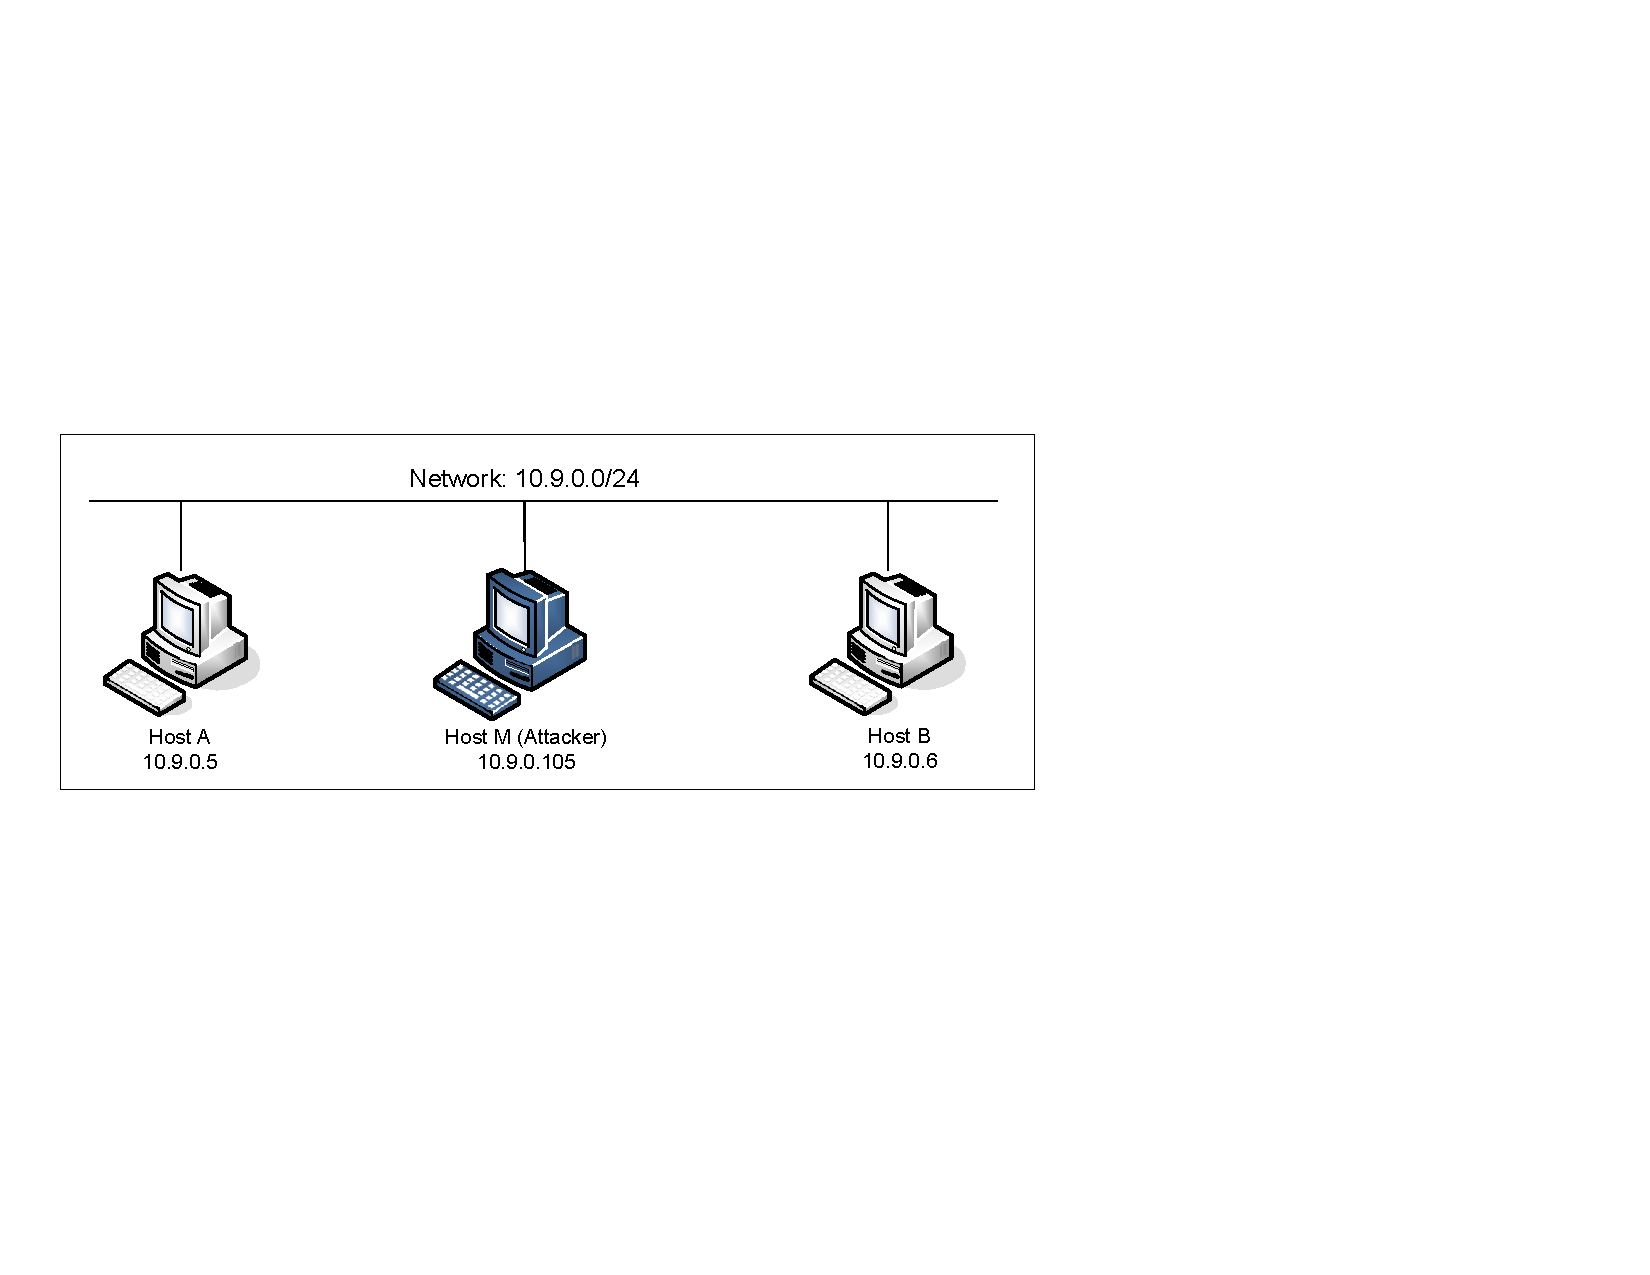
\includegraphics[width=0.8\textwidth]{\commonfolder/Figs/ARP_onelan.pdf}
\end{center}
\caption{Configuración del entorno}
\label{arp:fig:labsetup}
\end{figure}
 

% -------------------------------------------
% SUBSECTION
% -------------------------------------------
\subsection{Setup del Contenedor y sus Comandos}

%%%%%%%%%%%%%%%%%%%%%%%%%%%%%%%%%%%%%%%%%%%%
Para empezar a preparar el contenedor, deberá descargarse el archivo \texttt{Labsetup.zip} ubicado en el laboratorio correspondiente dentro del sitio web oficial y copiarlo dentro de la Máquina Virtual prevista por SEED. Una vez descargado deberá descomprimirlo y entrar dentro del directorio \texttt{Labsetup} donde encontrará el archivo \texttt{docker-compose.yml} que servirá para setear el entorno de laboratorio. Para una información más detallada sobre el archivo \texttt{Dockerfile} y otros archivos relacionados, puede encontrarla dentro del Manual de Usuario del laboratorio en uso, en el sitio web oficial de SEED.

Si esta es su primera experiencia haciendo el setup del laboratorio usando contenedores es recomendable que lea el manual anteriormente mencionado.

A continuación, se muestran los comandos más usados en Docker y Compose.
Debido a que estos comandos serán usados con mucha frecuencia, hemos creados un conjunto de alias para los mismos, ubicados en del archivo \texttt{.bashrc} dentro de la Máquina Virtual provista por SEED (Ubuntu 20.04)

\begin{lstlisting}
$ docker-compose build  # Build the container image
$ docker-compose up     # Start the container
$ docker-compose down   # Shut down the container

// Aliases for the Compose commands above
$ dcbuild       # Alias for: docker-compose build
$ dcup          # Alias for: docker-compose up
$ dcdown        # Alias for: docker-compose down
\end{lstlisting}


Dado que todos los contenedores estarán corriendo en un segundo plano. Necesitamos correr comandos para interactuar con los mismos, una de las operaciones fundamentales es obtener una shell en el contenedor. 
Para este propósito usaremos \texttt{"docker ps"} para encontrar el ID del contenedor deseado y ingresaremos \texttt{"docker exec"} para correr una shell en ese contenedor.
Hemos creado un alias para ello dentro del archivo \texttt{.bashrc}

\begin{lstlisting}
$ dockps        // Alias for: docker ps --format "{{.ID}}  {{.Names}}" 
$ docksh <id>   // Alias for: docker exec -it <id> /bin/bash

// The following example shows how to get a shell inside hostC
$ dockps
b1004832e275  hostA-10.9.0.5
0af4ea7a3e2e  hostB-10.9.0.6
9652715c8e0a  hostC-10.9.0.7

$ docksh 96
root@9652715c8e0a:/#  

// Note: If a docker command requires a container ID, you do not need to 
//       type the entire ID string. Typing the first few characters will 
//       be sufficient, as long as they are unique among all the containers. 
\end{lstlisting}

En caso de problemas configurando el entorno, por favor consulte la sección ``Common Problems'' en el manual ofrecido por SEED. 


%%%%%%%%%%%%%%%%%%%%%%%%%%%%%%%%%%%%%%%%%%%%


% -------------------------------------------
% SUBSECTION
% -------------------------------------------
\subsection{El contenedor de Ataque}

Para este laboratorio podemos usar tanto una Máquina Virtual como un contenedor como máquina de ataque. Si observa el archivo Docker Compose, verá que el contenedor de ataque está configurado de forma diferente al resto de los contenedores. Las diferencias son las siguientes:

\begin{itemize}
\item \textit{Directorio Compartido.} Cuando usemos el contenedor del atacante para realizar los ataques, necesitamos poner el código de ataque dentro del contenedor.

%%%%%%%%%%%%%%%%%%%%%%%%%%%%%%%%%%%%%%%%%%%%%%%
Code editing is more convenient inside the VM than in containers, 
because we can use our favorite editors.
In order for the VM and container to share files, 
we have created a shared folder between the VM and the container
using the Docker \texttt{volumes}.
If you look at the Docker Compose file, you will find out that
we have added the following entry to some of the containers.
It indicates mounting the \texttt{./volumes} folder on the host
machine (i.e., the VM) to the \texttt{/volumes} folder inside the container.
We will write our code in the \texttt{./volumes} folder (on the VM), so they
can be used inside the containers.

\begin{lstlisting}
volumes:
       - ./volumes:/volumes
\end{lstlisting}


%%%%%%%%%%%%%%%%%%%%%%%%%%%%%%%%%%%%%%%%%%%%%%%

\item \textit{Modo Privilegiado.}
%%%%%%%%%%%%%%%%%%%%%%%%%%%%%%%%%%%%%%%%%%%%%%%
Para poder modificar parámetros del kernel en tiempo de ejecución (usando  \texttt{sysctl}), tal como IP forwarding, el contenedor debe de ser privilegiado.
Esto se consigue incluyendo la siguiente entrada dentro del archivo Docker compose del contenedor.

\begin{lstlisting}
privileged: true
\end{lstlisting}


%%%%%%%%%%%%%%%%%%%%%%%%%%%%%%%%%%%%%%%%%%%%%%%

\end{itemize}


% -------------------------------------------
% SUBSECTION
% -------------------------------------------
\subsection{Sniffing de Paquetes} 

%%%%%%%%%%%%%%%%%%%%%%%%%%%%%%%%%%%%%%%%%%%%%%%

Poder hacer sniffing de paquetes es algo muy importante para este laboratorio, dado que si las cosas no resultan como se esperan, poder observar el trayecto de estos paquetes nos permitirá identificar determinados problemas.
Existen varias formas para hacer sniffing de paquetes:

\begin{itemize}
\item Corriendo \texttt{tcpdump} en los contenedores.
Hemos instalado la utilidad \texttt{tcpdump} en cada uno de los contenedores. Para poder sniffear los paquetes que viajan en una interfaz determinada, necesitamos como primer paso determinar cual es esa interfaz y hacer lo siguiente (assumiendo que el nombre de la interfaz es \texttt{eth0}):

\begin{lstlisting}
# tcpdump -i eth0 -n
\end{lstlisting}

Cabe aclarar que como estamos dentro de un contenedor, Docker implementa un mecanismo de isolación que sólo permite monitorear los paquetes que entran y salen del contenedor en donde se está ejecutando \texttt{tcpdump} por lo que no podremos hacer sniffing de paquetes entre contenedores.
Sin embargo, si un contenedor usa el modo \texttt{host} en su configuración de red, puede sniffear los paquetes de otros contenedores.

\item Corriendo \texttt{tcpdump} en la Máquina Virtual. Si corremos \texttt{tcpdump} dentro de la Máquina Virtual, no estamos sujetos a las mismas restricciones que impone Docker sobre sus contenedores, podemos hacer sniffing sobre todos los paquetes que entran y salen en los contenedores que se encuentran corriendo. La interfaz de red de la Máquina Virtual es diferente que la interfaz de los contenedores.
Generalmente en los contenedores cada interfaz empieza con \texttt{eth}; en la Máquina Virtual, la interfaz de red creada por Docker empieza con \texttt{br-}, seguido por el ID de red.
Puede usar el comando \texttt{ip address} para obtener el nombre de interfaz de la Máquina Virtual y de los contenedores.

\item También podemos usar Wireshark en la Máquina Virtual para sniffear paquetes. Al igual que \texttt{tcpdump}, necesitamos seleccionar en que interfaz Wireshark debería de estar escuchando para hacer el sniffing.
\end{itemize}


%%%%%%%%%%%%%%%%%%%%%%%%%%%%%%%%%%%%%%%%%%%%%%%



% *******************************************
% SECTION
% ******************************************* 
\section{Tarea 1: ARP Caché Poisoning}

El objetivo de esta tarea es poder hacer spoofing de paquetes para lanzar un ataque de ARP caché poisoning sobre una máquina, de tal forma que cuando dos máquinas víctimas A y B se traten de comunicar entre ellas, sus paquetes serán interceptados por el ataque, quién podra realizar cambios sobre los mismos y ser un man in the middle entre A y B. Este tipo de ataque es llamado Man-In-The-Middle (MITM).
En este laboratorio usaremos ARP caché poisoning para conducir un ataque MITM.

El siguiente código base muestra como construir un paquete ARP usando Scapy.
Por favor reemplace el nombre de la interfaz \texttt{br-05f0c56e8085} con la obtenida en su propia máquina (vea la sección anterior).

\begin{lstlisting}
#!/usr/bin/env python3
from scapy.all import *

E = Ether()
A = ARP()

pkt = E/A
sendp(pkt, iface='br-05f0c56e8085')
\end{lstlisting}

El programa anterior construye y envía un paquete ARP. Por favor complete con los valores necesarios para definir los atributos de su propio paquete ARP. Podemos usar \texttt{ls(ARP)} para ver los nombres de los atributos que posee la clase ARP. Si un campo no tiene valor, un valor por defecto será usado (vea la tercera columna del output):


\begin{lstlisting}
$ python3
>>> from scapy.all import *
>>> ls(ARP)
hwtype     : XShortField                         = (1)
ptype      : XShortEnumField                     = (2048)
hwlen      : ByteField                           = (6)
plen       : ByteField                           = (4)
op         : ShortEnumField                      = (1)
hwsrc      : ARPSourceMACField                   = (None)
psrc       : SourceIPField                       = (None)
hwdst      : MACField                            = ('00:00:00:00:00:00')
pdst       : IPField                             = ('0.0.0.0')
\end{lstlisting}

En esta tarea, tenemos tres máquinas (contenedores), A, B y M.
Queremos atacar la caché ARP de A, de tal manera que la IP de B sea mapeada en la dirección MAC de M. Podemos chequear la cache ARP de una máquina usando el siguiente comandop. Si quiere chequear la cache ARP asociada a una interfaz específica, puede usar el parámetro \texttt{-i}.

\begin{lstlisting}
$ arp -n
Address     HWtype  HWaddress           Flags Mask  Iface
10.0.2.1    ether   52:54:00:12:35:00   C           enp0s3
10.0.2.3    ether   08:00:27:48:f4:0b   C           enp0s3
\end{lstlisting}

Existen muchas formas de conducir un ataque de ARP caché poisoning. Los estudiantes deberán de intentar los siguientes métodos y reportar cuales funcionan y cuales no.

\begin{itemize}
\item \textbf{Tarea 1.A (Usando ARP Request).} En el Host M, construya un paquete ARP Request y envíelo al Host A. Vea la caché ARP del Host A y si la dirección MAC de M es mapeada en la dirección IP de B.

\item \textbf{Tarea 1.B (Usando ARP Reply).} En el Host M, construya un paquete ARP Reply y envíelo al Host A. Vea la caché ARP del Host A y si la dirección MAC de M es mapeada en la dirección IP de B.
Intente este ataque para los siguientes dos escenarios:

    \begin{itemize}
      \item Escenario 1: La dirección IP de B existe en la caché de A.
      \item Escenario 2: La dirección IP de B no existe en la caché de A.
    \end{itemize}
     
    
\item \textbf{Tarea 1C (Usando ARP gratuitous message).} En el Host M, construya un paquete ARP gratuitous message y envíelo al Host A. Vea la caché ARP del Host A y si la dirección MAC de M es mapeada en la dirección IP de B.  Por favor ejecute el ataque usando los dos escenarios que son decriptos en la Tarea 1.B.

ARP gratuitous es un tipo de paquete especial ARP Request. Este se usa cuando una máquina host necesita actualizar información que quedo desactualizada dentro de la caché ARP del resto de las máquinas. El paquete ARP gratuitous tiene las siguientes características:

\begin{itemize}
\item La dirección IP de origen y destino son las mismas, y pertenecen a la máquina que está emitindo el paquete ARP gratuitous.

\item Tanto en la cabecera ARP como en la cabecera Ethernet, la dirección MAC de destino es la dirección MAC de broadcast ({\tt ff:ff:ff:ff:ff:ff}).

\item No se espera respuesta.
\end{itemize}
\end{itemize}



% *******************************************
% SECTION
% ******************************************* 
\section{Tarea 2: Ataque MITM en Telnet Usando ARP Caché Poisoning}

Hosts A and B are communicating using Telnet, and Host M wants to intercept their
communication, so it can make changes to the data sent between A and B. The setup is depicted
in Figure~\ref{arp:fig:telnet_mitm}. We have already created an account called
\texttt{"seed"} inside the container, the password is \texttt{"dees"}. You can 
telnet into this account. 

\begin{figure}
    \centering
    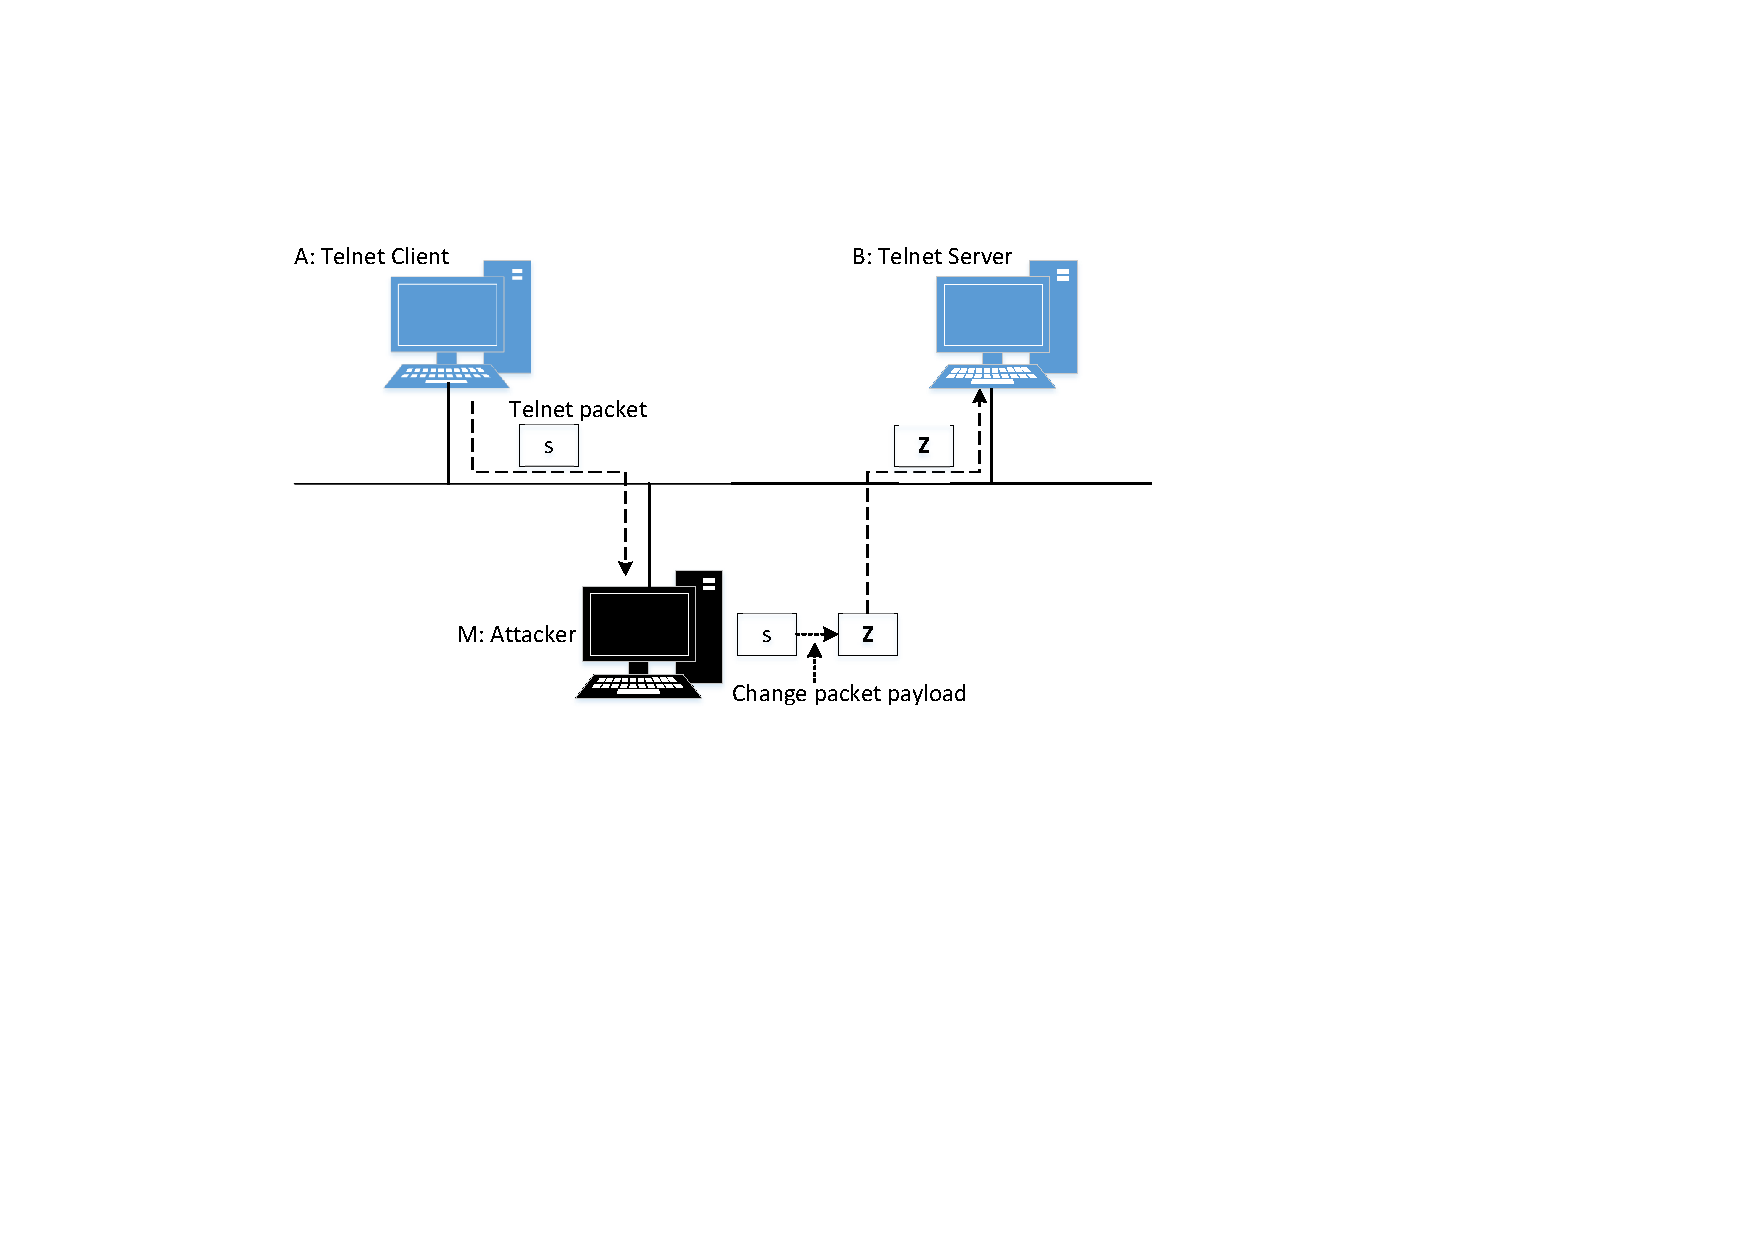
\includegraphics[width=0.8\textwidth]{\arpFigs/telnet_mitm.pdf}
    \caption{Ataque Man-In-The-Middle Attack contra telnet}
    \label{arp:fig:telnet_mitm}
\end{figure}


\paragraph{Paso 1 (Launch the ARP cache poisoning attack).} First, Host M conducts an ARP cache
poisoning attack on both A and B, such that in A's ARP cache, B's IP address maps to M's MAC
address, and in B's ARP cache, A's IP address also maps to M's MAC address. After this step,
packets sent between A and B will all be sent to M. We will use the ARP cache poisoning attack
from Task 1 to achieve this goal. It is better that you send out the spoofed packets
constantly (e.g. every 5 seconds); otherwise, the fake entries may be replaced by 
the real ones. 



\paragraph{Paso 2 (Testing).} After the attack is successful, please try to ping each other
between Hosts A and B, and report your observation. Please show Wireshark results in your
report. Before doing this step, please make sure that the IP forwarding on Host M is turned
off. You can do that with the following command:

\begin{lstlisting}
# sysctl net.ipv4.ip_forward=0
\end{lstlisting}

\paragraph{Paso 3 (Turn on IP forwarding).} Now we turn on the IP forwarding on Host M, so it
will forward the packets between A and B. Please run the following command and repeat Step 2.
Please describe your observation. 

\begin{lstlisting}
# sysctl net.ipv4.ip_forward=1
\end{lstlisting}

\paragraph{Paso 4 (Launch the MITM attack).} We are ready to make changes to the Telnet data
between A and B. Assume that A is the Telnet client and B is the Telnet server. After A has
connected to the Telnet server on B, for every key stroke typed in A's Telnet window, a TCP
packet is generated and sent to B. We would like to intercept the TCP packet, and replace each
typed character with a fixed character (say Z). This way, it does not matter what the user
types on A, Telnet will always display Z.

From the previous steps, we are able to redirect the TCP packets to Host M, but instead of
forwarding them, we would like to replace them with a spoofed packet. We will write a
sniff-and-spoof program to accomplish this goal. In particular, we would like to do the
following: 

\begin{itemize}

\item We first keep the IP forwarding on, so we can successfully create a Telnet connection
between A to B. Once the connection is established, we turn off the IP forwarding using the
following command. Please type something on A's Telnet window, and report your observation: 

\begin{lstlisting}
# sysctl net.ipv4.ip_forward=0
\end{lstlisting}

\item We run our sniff-and-spoof program on Host M, such that for the captured packets sent
from A to B,  we spoof a packet but with TCP different data. For packets from B to A (Telnet
response), we do not make any change, so the spoofed packet is exactly the same as the original
one. 
\end{itemize} 

To help students get started, we provide a skeleton sniff-and-spoof
program in the following. The program capture all the TCP packets, and 
then for packets from A to B, it makes some changes (the modification
part is not included, because that is part of the task). For packets from
B to A, the program does not make any change.  

\begin{lstlisting}
#!/usr/bin/env python3
from scapy.all import *

IP_A = "10.9.0.5"
MAC_A = "02:42:0a:09:00:05"
IP_B = "10.9.0.6"
MAC_B = "02:42:0a:09:00:06"


def spoof_pkt(pkt):
    if pkt[IP].src == IP_A and pkt[IP].dst == IP_B:
         # Create a new packet based on the captured one.
         # 1) We need to delete the checksum in the IP & TCP headers, 
         #    because our modification will make them invalid.
         #    Scapy will recalculate them if these fields are missing. 
         # 2) We also delete the original TCP payload.

         newpkt = IP(bytes(pkt[IP]))
         del(newpkt.chksum)
         del(newpkt[TCP].payload)
         del(newpkt[TCP].chksum)

         #################################################################
         # Construct the new payload based on the old payload.
         # Students need to implement this part.

         if pkt[TCP].payload:
             data = pkt[TCP].payload.load  # The original payload data
             newdata = data   # No change is made in this sample code

             send(newpkt/newdata)
         else:
             send(newpkt)
         ################################################################

    elif pkt[IP].src == IP_B and pkt[IP].dst == IP_A:
         # Create new packet based on the captured one 
         # Do not make any change 

         newpkt = IP(bytes(pkt[IP]))
         del(newpkt.chksum)
         del(newpkt[TCP].chksum)
         send(newpkt)


f = 'tcp'
pkt = sniff(iface='eth0', filter=f, prn=spoof_pkt)
\end{lstlisting}


It should be noted that the code above captures all the TCP 
packets, including the one generated by the program itself. That is 
undesirable, as it will affect
the performance. Students needs to change the filter, so it does not capture 
its own packets. 


\paragraph{Behavior of Telnet.}
In Telnet, typically, every character we type in the Telnet window triggers
an individual TCP packet, but if you type very fast, some characters may be 
sent together in the same packet. 
That is why in a typical Telnet packet from client to server, 
the payload only contains one character.  The
character sent to the server will be echoed back by the server, 
and the client will then display the
character in its window. Therefore, what we see in the client window is not the direct result
of the typing; whatever we type in the client window takes a round trip before it is displayed.
If the network is disconnected, whatever we typed on the client window will not displayed,
until the network is recovered. Similarly, if attackers change the character to Z during the
round trip, Z will be displayed at the Telnet client window, even though
that is not what you have typed.




% *******************************************
% SECTION
% ******************************************* 
\section{Tarea 3: Ataque MITM en Netcat Usando ARP Caché Poisoning}

This task is similar to Task 2, except that
Hosts A and B are communicating using \texttt{netcat}, instead of \texttt{telnet}.
Host M wants to intercept their
communication, so it can make changes to the data sent between A and B.
You can use the following commands to establish a \texttt{netcat} TCP
connection between A and B:


\begin{lstlisting}
On Host B (server, IP address is 10.9.0.6), run the following:
# nc -lp 9090

On Host A (client), run the following:
# nc 10.9.0.6 9090
\end{lstlisting}
 

Once the connection is made, you can type messages on A.
Each line of messages will be put into a TCP packet sent 
to B, which simply displays the message.  
Your task is to replace every occurrence of your first name in the 
message with a sequence of A's. The length of the sequence should be the 
same as that of your first name, or you will mess up the TCP sequence
number, and hence the entire TCP connection. You need to use your real
first name, so we know the work is done by you.  



% *******************************************
% SECTION
% ******************************************* 
\section{Informe del Laboratorio}


%%%%%%%%%%%%%%%%%%%%%%%%%%%%%%%%%%%%%%%%

Debe enviar un informe de laboratorio detallado, con capturas de pantalla, para describir lo que ha hecho y lo que ha observado.
También debe proporcionar una explicación a las observaciones que sean interesantes o sorprendentes.
Enumere también los fragmentos de código más importantes seguidos de una explicación. No recibirán créditos aquellos fragmentos de códigos que no sean explicados.
%%%%%%%%%%%%%%%%%%%%%%%%%%%%%%%%%%%%%%%%


% *******************************************
% SECTION
% *******************************************
\section*{Agradecimientos}

Este documento ha sido traducido al Español por Facundo Fontana



\end{document}



